% !TeX root = ../main.tex
% 第 1 章 测度与维数 (对应原书 pp. 1--19)

\chapter{测度与维数}

\section{基本测度论}

本节简明扼要地叙述我们所需要的基本测度论.更完整的论述可参见 \textcite{kingmantaylor1966} 或 \textcite{rogers1970}.

设 $X$ 为任意集合.(我们随后将取 $X$ 为 $n$ 维 Euclid 空间 $\mathbb{R}^n$.)称 $X$ 的子集的一个非空族 $\mathcal{S}$ 为 \newterm{sigma-field}{$\sigma$-域}{sigma-field}，如果 $\mathcal{S}$ 在取补与可数并下封闭（即若 $E\in\mathcal{S}$，则 $X\setminus E\in\mathcal{S}$；且若 $E_1,E_2,\ldots\in\mathcal{S}$，则 $\bigcup_{j=1}^{\infty}E_j\in\mathcal{S}$）.一点初等集合论表明，$\sigma$-域在可数交与集合差下也封闭，并且 $X$ 与空集 $\emptyset$ 属于 $\mathcal{S}$.

集合序列 $\{E_j\}$ 的\newterm{limit-lower}{下极限}{limit, lower}与\newterm{limit-upper}{上极限}{limit, upper}定义为
\[
  \varliminf_{j\to\infty}E_j=\bigcup_{k=1}^{\infty}\bigcap_{j=k}^{\infty}E_j
\]
与
\[
  \varlimsup_{j\to\infty}E_j=\bigcap_{k=1}^{\infty}\bigcup_{j=k}^{\infty}E_j.
\]
于是 $\varliminf E_j$ 由那些除有限多个 $E_j$ 之外都属于每个 $E_j$ 的点组成，而 $\varlimsup E_j$ 由那些属于无穷多个 $E_j$ 的点组成.由这些定义的形式显然可见，若每个 $E_j$ 都属于 $\sigma$-域 $\mathcal{S}$，则 $\varliminf E_j,\ \varlimsup E_j\in\mathcal{S}$.若 $\varliminf E_j=\varlimsup E_j$，则用 $\lim E_j$ 表示这个公共值；当 $\{E_j\}$ 为递增或递减集合序列时总会出现这种情形.

设 $\mathcal{C}$ 为 $X$ 的子集的任意族.称由 $\mathcal{C}$ \newterm{sigma-field-generated}{生成的 $\sigma$-域}{sigma-field generated by}，记作 $\mathcal{S}(\mathcal{C})$，为所有包含 $\mathcal{C}$ 的 $\sigma$-域之交.直接验证可知 $\mathcal{S}(\mathcal{C})$ 本身是一个 $\sigma$-域，可以视为包含 $\mathcal{C}$ 的``最小''的 $\sigma$-域.

\newterm{measure}{测度}{measure}是定义在 $X$ 的子集的某个 $\sigma$-域 $\mathcal{S}$ 上、取值于 $[0,\infty]$ 的函数 $\mu$，使得
\begin{equation}\label{eq:1.1}
  \mu(\emptyset)=0
\end{equation}
并且
\begin{equation}\label{eq:1.2}
  \mu\Bigl(\bigcup_{j=1}^{\infty}E_j\Bigr)=\sum_{j=1}^{\infty}\mu(E_j)
\end{equation}
对 $\mathcal{S}$ 中每个由两两不交的集合构成的可数序列 $\{E_j\}$ 成立.

由 \eqref{eq:1.2} 可知 $\mu$ 是递增的集合函数，即若 $E\subset E'$ 且 $E,E'\in\mathcal{S}$，则
\[
  \mu(E)\leq\mu(E').
\]

\begin{theorem}[\newterm{continuity-of-measures}{测度的连续性}{continuity of measures}]\label{thm:1.1}
设 $\mu$ 是 $X$ 的子集的 $\sigma$-域 $\mathcal{S}$ 上的测度.

(a) 若 $E_1\subset E_2\subset\cdots$ 是 $\mathcal{S}$ 中的递增集合序列，则
\[
  \mu\Bigl(\lim_{j\to\infty}E_j\Bigr)=\lim_{j\to\infty}\mu(E_j).
\]

(b) 若 $F_1\supset F_2\supset\cdots$ 是 $\mathcal{S}$ 中的递减集合序列且 $\mu(F_1)<\infty$，则
\[
  \mu\Bigl(\lim_{j\to\infty}F_j\Bigr)=\lim_{j\to\infty}\mu(F_j).
\]

(c) 对 $\mathcal{S}$ 中的任意集合序列 $\{F_j\}$，
\[
  \mu\Bigl(\varliminf_{j\to\infty}F_j\Bigr)\leq\varliminf_{j\to\infty}\mu(F_j).
\]
\end{theorem}

\begin{proof}
(a) 我们可以把 $\bigcup_{j=1}^{\infty}E_j$ 表为不交并 $E_1\cup\bigcup_{j=2}^{\infty}(E_j\setminus E_{j-1})$.于是由 \eqref{eq:1.2}，
\[
\begin{aligned}
  \mu\Bigl(\lim_{j\to\infty}E_j\Bigr)
    &=\mu\Bigl(\bigcup_{j=1}^{\infty}E_j\Bigr)
     =\mu(E_1)+\sum_{2}^{\infty}\mu(E_j\setminus E_{j-1})\\
    &=\lim_{k\to\infty}\Bigl[\mu(E_1)+\sum_{2}^{k}\mu(E_j\setminus E_{j-1})\Bigr]
     =\lim_{k\to\infty}\mu\Bigl(E_1\cup\bigcup_{2}^{k}(E_j\setminus E_{j-1})\Bigr)
     =\lim_{k\to\infty}\mu(E_k).
\end{aligned}
\]

(b) 若令 $E_j=F_1\setminus F_j$，则 $\{E_j\}$ 如 (a) 中所述.由于 $\bigcap_{j}F_j=F_1\setminus\bigcup_{j}E_j$，
\begin{align*}
  \mu\Bigl(\lim_{j\to\infty}F_j\Bigr)
  &=\mu\Bigl(\bigcap_{j=1}^{\infty}F_j\Bigr)
  =\mu(F_1)-\mu\Bigl(\bigcup_{j}E_j\Bigr)
  =\mu(F_1)-\lim_{j\to\infty}\mu(E_j)\\
  &=\lim_{j\to\infty}\bigl(\mu(F_1)-\mu(E_j)\bigr)
  =\lim_{j\to\infty}\mu(F_j).
\end{align*}

(c) 现在令 $E_k=\bigcap_{j=k}^{\infty}F_j$.则 $\{E_k\}$ 是 $\mathcal{S}$ 中的递增集合序列，故由 (a)，
\[
  \mu\Bigl(\lim_{j\to\infty}F_j\Bigr)
  =\mu\Bigl(\bigcup_{k=1}^{\infty}E_k\Bigr)
  =\lim_{k\to\infty}\mu(E_k)
  \leq\varliminf_{j\to\infty}\mu(F_j). \qedhere
\]
\end{proof}

接下来我们引入 \newterm{outer measure}{外测度}{outer measure}，它本质上是把性质 \eqref{eq:1.2} 减弱为次可加性的``测度''.确切地说，集合 $X$ 上的外测度 $\nu$ 是定义在 $X$ 的所有子集上、取值于 $[0,\infty]$ 的函数，使得
\begin{equation}\label{eq:1.3}
  \nu(\emptyset)=0,
\end{equation}
\begin{equation}\label{eq:1.4}
  \nu(A)\leq\nu(A')\qquad\text{若 } A\subset A',
\end{equation}
并且
\begin{equation}\label{eq:1.5}
  \nu\Bigl(\bigcup_{1}^{\infty}A_j\Bigr)\leq\sum_{1}^{\infty}\nu(A_j)
  \qquad\text{对 $X$ 的任意子集 } \{A_j\}.
\end{equation}

外测度之所以有用，是因为总存在一个子集的 $\sigma$-域，外测度在其上表现得如测度一般；对定义合理的外测度，这个 $\sigma$-域可以相当大.

称 $X$ 的子集 $E$ 为 \newterm{measurable set}{$\nu$-可测的}{measurable set}（即关于外测度 \newterm{outer-measurable}{可测}{outer measurable}），如果它对 $X$ 的每个子集都可加分解，即若
\begin{equation}\label{eq:1.6}
  \nu(A)=\nu(A\cap E)+\nu(A\setminus E)
\end{equation}
对所有``检验集''$A\subset X$ 成立.注意，为证集合 $E$ 是 $\nu$-可测的，只需验证
\begin{equation}\label{eq:1.7}
  \nu(A)\geq\nu(A\cap E)+\nu(A\setminus E),
\end{equation}
因为相反的不等式已含于 \eqref{eq:1.5} 中.显然可验证：若 $\nu(E)=0$，则 $E$ 是 $\nu$-可测的.

\begin{theorem}\label{thm:1.2}
设 $\nu$ 是一个外测度.$\nu$-可测集的族 $\mathcal{M}$ 构成一个 $\sigma$-域，且 $\nu$ 在 $\mathcal{M}$ 上的限制是一个测度.
\end{theorem}

\begin{proof}
显然 $\emptyset\in\mathcal{M}$，故 $\mathcal{M}$ 非空.又由 \eqref{eq:1.6} 的对称性，$A\in\mathcal{M}$ 当且仅当 $X\setminus A\in\mathcal{M}$，故 $\mathcal{M}$ 在取补下封闭.

为证 $\mathcal{M}$ 在可数并下封闭，设 $E_1,E_2,\ldots\in\mathcal{M}$，并设 $A$ 为任意集合.对 $E_1,E_2,\ldots$ 依次应用 \eqref{eq:1.6}，取相应的检验集，得
\[
\begin{aligned}
  \nu(A)
    &=\nu(A\cap E_1)+\nu(A\setminus E_1)\\
    &=\nu(A\cap E_1)+\nu\bigl((A\setminus E_1)\cap E_2\bigr)+\nu(A\setminus E_1\setminus E_2)\\
    &=\cdots\\
    &=\sum_{j=1}^{k}\nu\Bigl(\Bigl(A\setminus\bigcup_{i=1}^{j-1}E_i\Bigr)\cap E_j\Bigr)
      +\nu\Bigl(A\setminus\bigcup_{j=1}^{k}E_j\Bigr).
\end{aligned}
\]
于是
\[
  \nu(A)\geq\sum_{j=1}^{k}\nu\Bigl(\Bigl(A\setminus\bigcup_{i=1}^{j-1}E_i\Bigr)\cap E_j\Bigr)
  +\nu\Bigl(A\setminus\bigcup_{j=1}^{\infty}E_j\Bigr)
\]
对一切 $k$ 成立，从而
\begin{equation}\label{eq:1.8}
  \nu(A)\geq\sum_{j=1}^{\infty}\nu\Bigl(\Bigl(A\setminus\bigcup_{i=1}^{j-1}E_i\Bigr)\cap E_j\Bigr)
  +\nu\Bigl(A\setminus\bigcup_{j=1}^{\infty}E_j\Bigr).
\end{equation}
另一方面，
\[
  A\cap\bigcup_{j=1}^{\infty}E_j=\bigcup_{j=1}^{\infty}\Bigl(\Bigl(A\setminus\bigcup_{i=1}^{j-1}E_i\Bigr)\cap E_j\Bigr),
\]
故利用 \eqref{eq:1.5}，
\[
  \nu(A)\leq\nu\Bigl(A\cap\bigcup_{j=1}^{\infty}E_j\Bigr)+\nu\Bigl(A\setminus\bigcup_{j=1}^{\infty}E_j\Bigr)
  \leq\sum_{j=1}^{\infty}\nu\Bigl(\Bigl(A\setminus\bigcup_{i=1}^{j-1}E_i\Bigr)\cap E_j\Bigr)
  +\nu\Bigl(A\setminus\bigcup_{j=1}^{\infty}E_j\Bigr)\leq\nu(A),
\]
其中末一步用到 \eqref{eq:1.8}.由此得 $\bigcup_{j=1}^{\infty}E_j\in\mathcal{M}$，故 $\mathcal{M}$ 是一个 $\sigma$-域.

现在设 $E_1,E_2,\ldots$ 为 $\mathcal{M}$ 中两两不交的集合.在 \eqref{eq:1.8} 中取 $A=\bigcup_{j=1}^{\infty}E_j$，得
\[
  \nu\Bigl(\bigcup_{j=1}^{\infty}E_j\Bigr)\geq\sum_{j=1}^{\infty}\nu(E_j),
\]
再与 \eqref{eq:1.5} 结合，便知 $\nu$ 在 $\mathcal{M}$ 上是一个测度.
\end{proof}

称外测度 $\nu$ 是 \emph{正则的}\newterm{regular-outer-measure}{正则的}{regular outer measure}，若对每个集合 $A$ 都存在包含 $A$ 的 $\nu$-可测集 $E$，使得 $\nu(A)=\nu(E)$.

\begin{lemma}\label{lem:1.3}
若 $\nu$ 是正则外测度，$\{A_j\}$ 是任意递增集合序列，则
\[
  \lim_{j\to\infty}\nu(A_j)=\nu\Bigl(\lim_{j\to\infty}A_j\Bigr).
\]
\end{lemma}

\begin{proof}
对每个 $j$，选取 $\nu$-可测集 $E_j$ 使 $E_j\supset A_j$ 且 $\nu(E_j)=\nu(A_j)$.于是利用 \eqref{eq:1.4} 与 \cref{thm:1.1}(c)，
\[
  \nu\Bigl(\lim A_j\Bigr)=\nu\Bigl(\varliminf A_j\Bigr)\leq\nu\Bigl(\varliminf E_j\Bigr)\leq\varliminf\nu(E_j)=\lim\nu(A_j).
\]
相反的不等式由 \eqref{eq:1.4} 得出.
\end{proof}

现在设 $(X,d)$ 为度量空间.（就我们的目的而言，$X$ 通常为 $n$ 维 Euclid 空间 $\mathbb{R}^n$，$d$ 为通常的距离函数.）属于由 $X$ 的闭子集生成的 $\sigma$-域的集合称为该空间的 \newterm{Borel sets}{Borel 集}{Borel set}.Borel 集包括开集（作为闭集的补集）、\newterm{fsigma-set}{$F_{\sigma}$-集}{F$\sigma$-set}（即可数个闭集之并）、\newterm{gdelta-set}{$G_{\delta}$-集}{G$\delta$-set}（即可数个开集之交）等.

称 $X$ 上的外测度 $\nu$ 为 \newterm{metric outer measure}{度量外测度}{metric outer measure}，若只要 $E$ 与 $F$ \emph{正分离}（\newterm{positively separated}{正分离}{positively separated}），即只要
\[
  d(E,F)=\inf\{d(x,y):x\in E,\,y\in F\}>0,
\]
就有
\begin{equation}\label{eq:1.9}
  \nu(E\cup F)=\nu(E)+\nu(F).
\end{equation}
我们将证明，若 $\nu$ 是度量外测度，则 $\nu$-可测集的族包含 Borel 集.证明基于下述形式的 \newterm{caratheodory-lemma}{Carathéodory 引理}{Caratheodory's lemma}.

\begin{lemma}\label{lem:1.4}
设 $\nu$ 是 $(X,d)$ 上的度量外测度.设 $\{A_j\}_{1}^{\infty}$ 是 $X$ 的子集的递增序列，$A=\lim_{j\to\infty}A_j$，并设 $d(A_j,A\setminus A_{j+1})>0$ 对每个 $j$ 成立.则 $\nu(A)=\lim_{j\to\infty}\nu(A_j)$.
\end{lemma}

\begin{proof}
只需证明
\begin{equation}\label{eq:1.10}
  \nu(A)\leq\lim_{j\to\infty}\nu(A_j),
\end{equation}
因为相反的不等式由 \eqref{eq:1.4} 得出.令 $B_1=A_1$，$B_j=A_j\setminus A_{j-1}$（$j\geq 2$）.若 $j+2\leq i$，则 $B_j\subset A_j$ 且 $B_i\subset A\setminus A_{i-1}\subset A\setminus A_{j+1}$，故 $B_i$ 与 $B_j$ 正分离.于是，把 \eqref{eq:1.9} 应用 $(m-1)$ 次得
\[
  \nu\Bigl(\bigcup_{k=1}^{m}B_{2k-1}\Bigr)=\sum_{k=1}^{m}\nu(B_{2k-1}),\qquad
  \nu\Bigl(\bigcup_{k=1}^{m}B_{2k}\Bigr)=\sum_{k=1}^{m}\nu(B_{2k}).
\]
我们可以假定这两个级数都收敛——否则，由于 $\bigcup_{k=1}^{m}B_{2k-1}$ 与 $\bigcup_{k=1}^{m}B_{2k}$ 都含于 $A_{2m}$，将有 $\lim_{j\to\infty}\nu(A_j)=\infty$.于是
\[
  \nu(A)=\nu\Bigl(\bigcup_{j=1}^{\infty}A_j\Bigr)
  =\nu\Bigl(A_j\cup\bigcup_{k=j+1}^{\infty}B_k\Bigr)
  \leq\nu(A_j)+\sum_{k=j+1}^{\infty}\nu(B_k)
  \leq\lim_{i\to\infty}\nu(A_i)+\sum_{k=j+1}^{\infty}\nu(B_k).
\]
由于该级数当 $j\to\infty$ 时趋于 $0$，故 \eqref{eq:1.10} 得证.
\end{proof}

\begin{theorem}\label{thm:1.5}
若 $\nu$ 是 $(X,d)$ 上的度量外测度，则 $X$ 的所有 Borel 子集都是 $\nu$-可测的.
\end{theorem}

\begin{proof}
由于 $\nu$-可测集构成一个 $\sigma$-域，而 Borel 集是含 $X$ 的闭子集的最小 $\sigma$-域，故只需证当 $E$ 为闭集、$A$ 为任意集合时 \eqref{eq:1.7} 成立.

设 $A_j$ 为 $A\setminus E$ 中与 $E$ 的距离至少为 $1/j$ 的点的集合.则 $d(A\cap E,A_j)\geq 1/j$，故
\begin{equation}\label{eq:1.11}
  \nu(A\cap E)+\nu(A_j)=\nu\bigl((A\cap E)\cup A_j\bigr)\leq\nu(A)
\end{equation}
对每个 $j$ 成立，因为 $\nu$ 是度量外测度.集合序列 $\{A_j\}$ 递增，且由于 $E$ 闭，$A\setminus E=\bigcup_{j=1}^{\infty}A_j$.于是，只要 $d(A_j,A\setminus E\setminus A_{j+1})>0$ 对一切 $j$ 成立，\cref{lem:1.4} 便给出 $\nu(A\setminus E)\leq\lim_{j\to\infty}\nu(A_j)$，再由 \eqref{eq:1.11} 即得 \eqref{eq:1.7}.但若 $x\in A\setminus E\setminus A_{j+1}$，则存在 $z\in E$ 使 $d(x,z)<1/(j+1)$，于是当 $y\in A_j$ 时
\[
  d(x,y)\geq d(y,z)-d(x,z)>1/j-1/(j+1)>0.
\]
故 $d(A_j,A\setminus E\setminus A_{j+1})>0$，如所需.
\end{proof}

还有一类重要的集合，与 Borel 集不同，它们由闭集的并与交显式地定义.若 $(X,d)$ 是度量空间，则 \newterm{Souslin sets}{Souslin 集}{Souslin set} 是如下形式的集合：
\[
  E=\bigcup_{i_1i_2\ldots}\ \bigcap_{k=1}^{\infty}E_{i_1i_2\ldots i_k},
\]
其中对每个由正整数构成的有限序列 $\{i_1,i_2,\ldots,i_k\}$，$E_{i_1i_2\ldots i_k}$ 都是闭集.注意，尽管 $E$ 由可数多个闭集构造而成，但其中的并是对连续统多个整数无穷序列取的.（每个闭集在该表达式中出现许多次.）

可以证明每个 Borel 集都是 Souslin 集，而且若底度量空间完备，则 Souslin 集的任何连续像仍是 Souslin 集.此外，若 $\nu$ 是度量空间 $(X,d)$ 上的外测度，则只要闭集都 $\nu$-可测，Souslin 集也就都 $\nu$-可测.由 \cref{thm:1.5} 可得：若 $\nu$ 是 $(X,d)$ 上的度量外测度，则 Souslin 集是 $\nu$-可测的.我们只顺带提及 Souslin 集.其测度论方面的更详细论述见 \textcite{rogers1970}，行家还可参阅 \textcites{rogers1980}.

\section{Hausdorff 测度}


从本书余下部分起，我们在 $n$ 维 Euclid 空间 $\mathbb{R}^n$ 中工作，不过应当强调，这里所说的许多内容在一般度量空间的框架下同样成立.

若 $U$ 是 $\mathbb{R}^n$ 的非空子集，我们定义 $U$ 的\newterm{diameter}{直径}{diameter}为 $|U|=\sup\{|x-y|:x,y\in U\}$.若 $E\subset\bigcup_{i}U_i$ 且 $0<|U_i|\leq\delta$ 对每个 $i$ 成立，则称 $\{U_i\}$ 为 $E$ 的一个 \newterm{delta-cover}{$\delta$-覆盖}{$\delta$-cover}.

设 $E\subset\mathbb{R}^n$，$s$ 为非负数.对 $\delta>0$ 定义
\begin{equation}\label{eq:1.12}
  \mathcal{H}^s_{\delta}(E)=\inf\sum_{i=1}^{\infty}|U_i|^s,
\end{equation}
其中下确界取遍 $E$ 的所有（可数）$\delta$-覆盖 $\{U_i\}$.容易验证 $\mathcal{H}^s_{\delta}$ 是 $\mathbb{R}^n$ 上的外测度.

为得到 $E$ 的 Hausdorff $s$ 维\newterm{hausdorff-outer-measure}{外测度}{Hausdorff outer measure}，令 $\delta\to 0$，即
\begin{equation}\label{eq:1.13}
  \mathcal{H}^{s}(E)=\lim_{\delta\to 0}\mathcal{H}^{s}_{\delta}(E)=\sup_{\delta>0}\mathcal{H}^{s}_{\delta}(E).
\end{equation}
该极限存在（但可能为无穷），因为当 $\delta$ 减小时 $\mathcal{H}^s_{\delta}$ 增大.易见 $\mathcal{H}^s$ 是外测度，而且它还是度量外测度.事实上，若 $\delta$ 小于正分离的集合 $E$ 与 $F$ 之间的距离，则 $E\cup F$ 的 $\delta$-覆盖中的任何集合都不能同时与 $E$ 和 $F$ 相交，于是
\[
  \mathcal{H}^s_{\delta}(E\cup F)=\mathcal{H}^s_{\delta}(E)+\mathcal{H}^s_{\delta}(F),
\]
从而对 $\mathcal{H}^s$ 也有类似的等式.$\mathcal{H}^s$ 在 $\mathcal{H}^s$-可测集构成的 $\sigma$-域上的限制称为 \newterm{Hausdorff measure}{Hausdorff $s$ 维测度}{Hausdorff measure}；由 \cref{thm:1.5}，该 $\sigma$-域包含 Borel 集（事实上还包含 Souslin 集）.

注意，若把 \eqref{eq:1.12} 中的下确界改为取遍 $E$ 的由凸集构成的 $\delta$-覆盖而非任意集合的 $\delta$-覆盖，则得到 Hausdorff 测度的一个等价定义，因为任何集合都含于一个同直径的凸集之中.类似地，取开集或取闭集构成的 $\delta$-覆盖有时也很方便.在各种情形下，尽管对 $\delta>0$ 所得的 $\mathcal{H}^s_{\delta}$ 的值可能不同，但极限 $\mathcal{H}^s$ 的值是一样的，见 \textcite{davies1956}.（然而，若下确界取遍由球构成的 $\delta$-覆盖，则会得到一个不同的测度；\textcite{besicovitch1928a} 第 3 章把这类``\newterm{spherical-hausdorff-measure}{球面 Hausdorff 测度}{Hausdorff measure, spherical}''与 Hausdorff 测度作了比较.）

对任意 $E$，显然当 $s$ 从 $0$ 增到 $\infty$ 时 $\mathcal{H}^s(E)$ 不增.此外，若 $s<t$，则
\[
  \mathcal{H}^s_{\delta}(E)\geq\delta^{s-t}\,\mathcal{H}^t_{\delta}(E),
\]
由此可得：若 $\mathcal{H}^t(E)$ 为正，则 $\mathcal{H}^s(E)$ 为无穷.于是存在唯一的值 $\dim E$，称为 $E$ 的 \newterm{Hausdorff dimension}{Hausdorff 维数}{Hausdorff dimension}，使得
\begin{equation}\label{eq:1.14}
  \mathcal{H}^{s}(E)=\infty\ \ \text{若}\ 0\leq s<\dim E,
  \qquad
  \mathcal{H}^{s}(E)=0\ \ \text{若}\ \dim E<s<\infty.
\end{equation}

若 $C$ 是 $\mathbb{R}^n$ 中边长为 $1$ 的方体，则用显然的方式把 $C$ 分成 $k^n$ 个边长为 $1/k$ 的小方体即可看出：若 $\delta\geq k^{-1}n^{\frac{1}{2}}$，则
\[
  \mathcal{H}^n_{\delta}(C)\leq k^{n}\bigl(k^{-1}n^{\frac{1}{2}}\bigr)^{n}\leq n^{\frac{1}{2}n},
\]
从而 $\mathcal{H}^n(C)<\infty$.于是当 $s>n$ 时 $\mathcal{H}^s(C)=0$，并且由于 $\mathbb{R}^n$ 可表示为可数多个这类方体之并，$\mathcal{H}^s(\mathbb{R}^n)=0$.由此可知对任意 $E\subset\mathbb{R}^n$ 有 $0\leq\dim E\leq n$.同样显然，若 $E\subset E'$，则 $\dim E\leq\dim E'$.

若 $\mathcal{H}^s$-可测集 $E\subset\mathbb{R}^n$ 满足 $0<\mathcal{H}^s(E)<\infty$，则称 $E$ 为一个 \newterm{s-set}{$s$-集}{$s$-set}；$1$-集有时也称为\newterm{linearly-measurable-set}{线性可测集}{linearly measurable set}.显然，$s$-集的 Hausdorff 维数等于 $s$，但重要的是要认识到，$s$-集远比 Hausdorff 维数为 $s$ 的可测集特殊.事实上，\textcite{besicovitch1942} 证明了任何集合都可以表示为连续统多个同维数集合的不交并.本书的大部分内容致力于研究 $s$-集的几何性质.

把 \eqref{eq:1.12} 中的 $|U_i|^s$ 换成 $h(|U_i|)$（其中 $h$ 是某个右连续的递增正函数），便得到 Hausdorff 测度定义的推广.我们的许多结果对这些更一般的测度都有直接的类似物，不过有时以代数上的简洁性为代价.此时集合 $E$ 的 Hausdorff``维数''可以更确切地理解为对函数的一个分划：一类函数使 $E$ 的测度为零，另一类使其为无穷（见 \textcite{rogers1970}）.若把 $|U_i|^s$ 换成 $h(U_i)$，其中 $h$ 只是集合 $U_i$ 的函数，甚至也能得到某些进展（见 \textcites{davies1969,daviessamuels1974}）.

下面我们证明 $\mathcal{H}^s$ 是正则测度，以及一个有用的推论：$s$-集可以从下方用闭子集逼近.这一证明由 \textcite{besicovitch1938} 给出，他还在 \citeyear{besicovitch1954} 证明了 \cref{thm:1.6}(b) 中有限性条件的必要性.

\begin{theorem}\label{thm:1.6}
(a) 若 $E$ 是 $\mathbb{R}^n$ 的任意子集，则存在包含 $E$ 的 $G_{\delta}$-集 $G$ 使 $\mathcal{H}^s(G)=\mathcal{H}^s(E)$.特别地，$\mathcal{H}^s$ 是正则外测度.

(b) 任何 $\mathcal{H}^s$-可测且 $\mathcal{H}^s$-测度有限的集合都包含一个测度相等的 $F_{\sigma}$-集，从而包含一个与它之差的测度可任意小的闭集.
\end{theorem}

\begin{proof}
(a) 若 $\mathcal{H}^s(E)=\infty$，则 $\mathbb{R}^n$ 就是测度相等之开集，故设 $\mathcal{H}^s(E)<\infty$.对每个 $i=1,2,\ldots$，选取 $E$ 的开 $2/i$-覆盖 $\{U_{ij}\}_j$ 使
\[
  \sum_{j=1}^{\infty}|U_{ij}|^s<\mathcal{H}^s_{1/i}(E)+1/i.
\]
则 $E\subset G$，其中 $G=\bigcap_{i=1}^{\infty}\bigcup_{j=1}^{\infty}U_{ij}$ 是一个 $G_{\delta}$-集.由于 $\{U_{ij}\}_j$ 是 $G$ 的 $2/i$-覆盖，$\mathcal{H}^s_{2/i}(G)\leq\mathcal{H}^s_{1/i}(E)+1/i$，令 $i\to\infty$ 即得 $\mathcal{H}^s(E)=\mathcal{H}^s(G)$.由于 $G_{\delta}$-集是 $\mathcal{H}^s$-可测的，故 $\mathcal{H}^s$ 是正则外测度.

(b) 设 $E$ 为 $\mathcal{H}^s$-可测且 $\mathcal{H}^s(E)<\infty$.利用 (a)，可找到包含 $E$ 的开集 $O_1,O_2,\ldots$，使得
\[
  \mathcal{H}^s\Bigl(\bigcap_{i=1}^{\infty}O_i\setminus E\Bigr)
  =\mathcal{H}^s\Bigl(\bigcap_{i=1}^{\infty}O_i\Bigr)-\mathcal{H}^s(E)=0.
\]
$\mathbb{R}^n$ 的任何开子集都是 $F_{\sigma}$-集，故设对每个 $i$ 有 $O_i=\bigcup_{j=1}^{\infty}F_{ij}$，其中 $\{F_{ij}\}_j$ 是递增的闭集序列.于是由 $\mathcal{H}^s$ 的连续性，
\[
  \lim_{j\to\infty}\mathcal{H}^s(E\cap F_{ij})=\mathcal{H}^s(E\cap O_i)=\mathcal{H}^s(E).
\]
因此，给定 $\varepsilon>0$，可找到 $j_i$ 使
\[
  \mathcal{H}^s(E\setminus F_{ij_i})<2^{-i}\varepsilon\qquad(i=1,2,\ldots).
\]
若 $F$ 为闭集 $\bigcap_{i=1}^{\infty}F_{ij_i}$，则
\[
  \mathcal{H}^s(F)\geq\mathcal{H}^s(E\cap F)\geq\mathcal{H}^s(E)-\sum_{i=1}^{\infty}\mathcal{H}^s(E\setminus F_{ij_i})>\mathcal{H}^s(E)-\varepsilon.
\]
由于 $F\subset\bigcap_{i=1}^{\infty}O_i$，故 $\mathcal{H}^s(F\setminus E)\leq\mathcal{H}^s\bigl(\bigcap_{i=1}^{\infty}O_i\setminus E\bigr)=0$.由 (a)，$F\setminus E$ 含于某个满足 $\mathcal{H}^s(G)=0$ 的 $G_{\delta}$-集 $G$.于是 $F\setminus G$ 是含于 $E$ 的 $F_{\sigma}$-集，且
\[
  \mathcal{H}^s(F\setminus G)\geq\mathcal{H}^s(F)-\mathcal{H}^s(G)>\mathcal{H}^s(E)-\varepsilon.
\]
对 $\varepsilon=\frac{1}{2},\frac{1}{3},\frac{1}{4},\ldots$ 取这样的 $F_{\sigma}$-集的可数并，便得到含于 $E$ 且与 $E$ 测度相等的 $F_{\sigma}$-集.
\end{proof}

下一条引理断言：任何用足够小的集合构成的覆盖去估计一个集合的 Hausdorff 测度的尝试，所得结果都不会比实际的 Hausdorff 测度小太多.

\begin{lemma}\label{lem:1.7}
设 $E$ 为 $\mathcal{H}^s$-可测且 $\mathcal{H}^s(E)<\infty$，$\varepsilon>0$.则存在只依赖于 $E$ 与 $\varepsilon$ 的 $\rho>0$，使得对任何满足 $0<|U_i|\leq\rho$ 的 Borel 集族 $\{U_i\}_{i=1}^{\infty}$ 有
\[
  \mathcal{H}^{s}\Bigl(E\cap\bigcup_{i}U_i\Bigr)<\sum_{i}|U_i|^{s}+\varepsilon.
\]
\end{lemma}

\begin{proof}
由 $\mathcal{H}^s$ 作为 $\mathcal{H}^s_{\delta}$ 当 $\delta\to 0$ 时极限的定义，可选取 $\rho$ 使得对 $E$ 的任何 $\rho$-覆盖 $\{W_i\}$ 有
\begin{equation}\label{eq:1.15}
  \mathcal{H}^{s}(E)<\sum|W_i|^{s}+\tfrac{1}{2}\varepsilon.
\end{equation}
给定满足 $0<|U_i|\leq\rho$ 的 Borel 集 $\{U_i\}$，可找到 $E\setminus\bigcup_{i}U_i$ 的 $\rho$-覆盖 $\{V_i\}$ 使
\[
  \mathcal{H}^{s}\Bigl(E\setminus\bigcup_{i}U_i\Bigr)+\tfrac{1}{2}\varepsilon>\sum|V_i|^{s}.
\]
由于 $\{U_i\}\cup\{V_i\}$ 便是 $E$ 的一个 $\rho$-覆盖，故由 \eqref{eq:1.15}
\[
  \mathcal{H}^{s}(E)<\sum|U_i|^{s}+\sum|V_i|^{s}+\tfrac{1}{2}\varepsilon.
\]
从而
\[
  \mathcal{H}^{s}\Bigl(E\cap\bigcup_{i}U_i\Bigr)
  =\mathcal{H}^{s}(E)-\mathcal{H}^{s}\Bigl(E\setminus\bigcup_{i}U_i\Bigr)
  <\sum|U_i|^{s}+\sum|V_i|^{s}+\tfrac{1}{2}\varepsilon-\sum|V_i|^{s}+\tfrac{1}{2}\varepsilon
  =\sum|U_i|^{s}+\varepsilon. \qedhere
\]
\end{proof}

本节最后，我们证明一个关于``一致 Lipschitz''映射所联系的集合的测度的简单引理.

\begin{lemma}\label{lem:1.8}
设 $\psi:E\to F$ 为满射，且对常数 $c$ 满足
\[
  |\psi(x)-\psi(y)|\leq c\,|x-y|\qquad(x,y\in E).
\]
则 $\mathcal{H}^s(F)\leq c^s\mathcal{H}^s(E)$.
\end{lemma}

\begin{proof}
对每个 $i$ 有 $|\psi(U_i\cap E)|\leq c\,|U_i|$.于是若 $\{U_i\}$ 是 $E$ 的 $\delta$-覆盖，则 $\{\psi(U_i\cap E)\}$ 是 $F$ 的 $c\delta$-覆盖.又 $\sum_{i}|\psi(U_i\cap E)|^s\leq c^s\sum_{i}|U_i|^s$，故 $\mathcal{H}^s_{c\delta}(F)\leq c^s\mathcal{H}^s_{\delta}(E)$，令 $\delta\to 0$ 即得结论.
\end{proof}

\section{覆盖结果}

Vitali 覆盖定理是几何测度论中最有用的工具之一.给定覆盖某集合 $E$ 的一个``足够大''的集合族，Vitali 定理从中选出一个不交子族，使之覆盖 $E$ 的几乎全部.

我们在下一条引理中阐述 Vitali 结果之证明所体现的基本原理，不过是在一个简化的场景中.称一个集合族是\newterm{semidisjoint}{半不交的}{semidisjoint}，若族中没有任何成员包含于另一个不同的成员.

\begin{lemma}\label{lem:1.9}
设 $\mathcal{C}$ 是含于 $\mathbb{R}^n$ 的有界子集中的一族球.则可找到有限或可数的不交子族 $\{B_i\}$，使得
\begin{equation}\label{eq:1.16}
  \bigcup_{B\in\mathcal{C}}B\subset\bigcup_{i}B_i',
\end{equation}
其中 $B_i'$ 是与 $B_i$ 同心、半径为其 $5$ 倍的球.此外，可使族 $\{B_i'\}$ 为半不交的.
\end{lemma}

\begin{proof}
我们归纳地选取 $\{B_i\}$.令 $d_0=\sup\{|B|:B\in\mathcal{C}\}$，并从 $\mathcal{C}$ 中选取满足 $|B_1|\geq\frac{1}{2}d_0$ 的 $B_1$.设 $B_1,\ldots,B_m$ 已经选定，令 $d_m=\sup\{|B|:B\in\mathcal{C},\ B\ \text{与}\ \bigcup_{1}^{m}B_i\ \text{不交}\}$.若 $d_m=0$，过程终止.否则，从 $\mathcal{C}$ 中选取与 $\bigcup_{1}^{m}B_i$ 不交且 $|B_{m+1}|\geq\frac{1}{2}d_m$ 的 $B_{m+1}$.这些球当然不交；我们断言它们还有所需的覆盖性质.设 $B\in\mathcal{C}$，则要么 $B=B_i$ 对某个 $i$ 成立，要么 $B$ 与某个满足 $2|B_i|\geq|B|$ 的 $B_i$ 相交.若非如此，$B$ 本应先于第一个满足 $2|B_m|<|B|$ 的球 $B_m$ 被选出.（注意，把体积求和可知 $\sum|B_i|^n<\infty$，故若选出了无穷多个球，则当 $i\to\infty$ 时 $|B_i|\to 0$.）无论哪种情形都有 $B\subset B_i'$，即得 \eqref{eq:1.16}.为使 $\{B_i'\}$ 半不交，只需在 $B_i'\subset B_j'$（对某个 $j\neq i$）时把 $B_i$ 从子族中去掉即可，注意 $B_i'$ 只能含于有限多个 $B_j'$.
\end{proof}

称集合族 $\mathcal{V}$ 是 $E$ 的一个 \newterm{Vitali class}{Vitali 类}{Vitali class}，若对每个 $x\in E$ 与 $\delta>0$，存在 $U\in\mathcal{V}$ 使 $x\in U$ 且 $0<|U|\leq\delta$.


\begin{theorem}[\newterm{vitali-covering-theorem}{Vitali 覆盖定理}{Vitali covering theorem}]\label{thm:1.10}
(a) 设 $E$ 是 $\mathbb{R}^n$ 的 $\mathcal{H}^s$-可测子集，$\mathcal{V}$ 是 $E$ 的由闭集构成的 Vitali 类.则可从 $\mathcal{V}$ 中选出（有限或可数的）不交序列 $\{U_i\}$，使得或者 $\sum|U_i|^s=\infty$，或者 $\mathcal{H}^s\bigl(E\setminus\bigcup_{i}U_i\bigr)=0$.

(b) 若 $\mathcal{H}^s(E)<\infty$，则给定 $\varepsilon>0$，还可要求
\[
  \mathcal{H}^{s}(E)\leq\sum_{i}|U_i|^{s}+\varepsilon.
\]
\end{theorem}

\begin{proof}
固定 $\rho>0$；不妨设对所有 $U\in\mathcal{V}$ 有 $|U|\leq\rho$.归纳地选取 $\{U_i\}$.令 $U_1$ 为 $\mathcal{V}$ 的任一成员.设 $U_1,\ldots,U_m$ 已经选定，令 $d_m$ 为 $\mathcal{V}$ 中那些与 $U_1,\ldots,U_m$ 都不交的 $U$ 的 $|U|$ 的上确界.若 $d_m=0$，则 $E\subset\bigcup_{1}^{m}U_i$，于是 (a) 得证，过程终止.否则，令 $U_{m+1}$ 为 $\mathcal{V}$ 中与 $\bigcup_{1}^{m}U_i$ 不交且 $|U_{m+1}|\geq\frac{1}{2}d_m$ 的集合.

设过程无限进行下去且 $\sum|U_i|^s<\infty$.对每个 $i$，令 $B_i$ 为圆心在 $U_i$ 中、半径为 $3|U_i|$ 的球.我们断言对每个 $k>1$，
\begin{equation}\label{eq:1.17}
  E\setminus\bigcup_{1}^{k}U_i\subset\bigcup_{k+1}^{\infty}B_i.
\end{equation}
事实上，若 $x\in E\setminus\bigcup_{1}^{k}U_i$，则存在不与 $U_1,\ldots,U_k$ 相交且 $x\in U$ 的 $U\in\mathcal{V}$.由于 $|U_i|\to 0$，存在 $m$ 使 $|U|>2|U_m|$.由 $\{U_i\}$ 的选取方法，$U$ 必与某个满足 $k<i<m$ 且 $|U|\leq 2|U_i|$ 的 $U_i$ 相交.由初等几何 $U\subset B_i$，故得 \eqref{eq:1.17}.于是若 $\delta>0$，只要 $k$ 大到足以保证对 $i>k$ 有 $|B_i|\leq\delta$，便有
\[
  \mathcal{H}^{s}_{\delta}\Bigl(E\setminus\bigcup_{1}^{\infty}U_i\Bigr)
  \leq\mathcal{H}^{s}_{\delta}\Bigl(E\setminus\bigcup_{1}^{k}U_i\Bigr)
  \leq\sum_{k+1}^{\infty}|B_i|^{s}
  =6^{s}\sum_{k+1}^{\infty}|U_i|^{s}.
\]
从而对一切 $\delta>0$ 有 $\mathcal{H}^s_{\delta}\bigl(E\setminus\bigcup_{1}^{\infty}U_i\bigr)=0$，故 $\mathcal{H}^s\bigl(E\setminus\bigcup_{1}^{\infty}U_i\bigr)=0$，即 (a) 得证.

为证 (b)，不妨设证明开始时选取的 $\rho$ 就是 \cref{lem:1.7} 中对应于 $\varepsilon$ 与 $E$ 的那个数.若 $\sum|U_i|^s=\infty$，则 (b) 显然.否则，由 (a) 与 \cref{lem:1.7},
\[
  \mathcal{H}^{s}(E)
  =\mathcal{H}^{s}\Bigl(E\setminus\bigcup_{i}U_i\Bigr)+\mathcal{H}^{s}\Bigl(E\cap\bigcup_{i}U_i\Bigr)
  =0+\mathcal{H}^{s}\Bigl(E\cap\bigcup_{i}U_i\Bigr)
  <\sum|U_i|^{s}+\varepsilon. \qedhere
\]
\end{proof}

\newterm{covering-theorems}{覆盖定理}{covering theorems}本身也得到了广泛的研究，它在调和分析以及几何测度论中都具有特殊的重要性.de Guzmán（\citeyear{deguzman1975,deguzman1981}） 的两本书描述了针对非常一般的集合类与测度类的结果，书中还包含进一步的文献.覆盖原理的一种处理方法归功于 Besicovitch（\citeyear{besicovitch1945a,besicovitch1946,besicovitch1947}）；其中第一篇文章包含了对密度（如本书 2.2~节所描述的）的应用.

\section{勒贝格测度}

我们把 \newterm{lebesgue-measure}{勒贝格测度}{Lebesgue measure}作为 $\mathbb{R}^n$ 中\newterm{volume}{体积}{volume}的通常定义的推广而得到（``体积''在 $\mathbb{R}^1$ 中指长度，在 $\mathbb{R}^2$ 中指面积）.

设 $C$ 是 $\mathbb{R}^n$ 中如下形式的\newterm{coordinate-block}{坐标块}{coordinate block}：
\[
  C=[a_1,b_1)\times[a_2,b_2)\times\cdots\times[a_n,b_n),
\]
其中对每个 $i$ 有 $a_i<b_i$.按显然的方式定义 $C$ 的体积为
\[
  V(C)=(b_1-a_1)(b_2-a_2)\cdots(b_n-a_n).
\]
设 $E\subset\mathbb{R}^n$，令
\begin{equation}\label{eq:1.18}
  \mathcal{L}^{n}(E)=\inf\sum_{i}V(C_i),
\end{equation}
其中下确界取遍 $E$ 的所有由块构成的序列 $\{C_i\}$ 的覆盖.易见 $\mathcal{L}^n$ 是 $\mathbb{R}^n$ 上的外测度，称为\newterm{lebesgue-outer-measure}{勒贝格外测度}{Lebesgue outer measure}.进一步，若 $E$ 是任一块，则 $\mathcal{L}^n(E)$ 与 $E$ 的体积一致；这只需把 \eqref{eq:1.18} 中的和用有限和逼近，再用包含 $C_i$ 之面的平面剖分 $E$ 即得.由于任何块 $C_i$ 都可以剖分成小子块而使 \eqref{eq:1.18} 中的和不变，故对任意 $\delta>0$，把下确界取遍 $E$ 的 $\delta$-覆盖即可.因而 $\mathcal{L}^n$ 是 $\mathbb{R}^n$ 上的度量外测度.$\mathcal{L}^n$ 在 $\mathcal{L}^n$-可测集（即勒贝格可测集，由 \cref{thm:1.5} 它包含 Borel 集）上的限制称为勒贝格 $n$ 维测度或\newterm{n-dim-lebesgue-measure}{体积}{n-dimensional Lebesgue measure}.

显然，$\mathbb{R}^1$ 上 $\mathcal{L}^1$ 与 $\mathcal{H}^1$ 的定义一致.可以预期，当 $n>1$ 时 $\mathbb{R}^n$ 上的外测度 $\mathcal{L}^n$ 与 $\mathcal{H}^n$ 也有联系；事实上它们只差一个常数倍.为说明这一点，我们需要下述著名的几何结果——``等直径不等式''（\newterm{isodiametric inequality}{等直径不等式}{isodiametric inequality}），即给定直径时体积最大的集合是球.利用对称化或其他方法的证明可在任何关于凸性的书中找到，例如 \textcite{eggleston1958}；另见\cref{exe:1.6}.

\begin{theorem}\label{thm:1.11}
直径为 $d$ 的闭凸集的 $n$ 维体积至多为 $\pi^{\frac{1}{2}n}\bigl(\tfrac{1}{2}d\bigr)^{n}/\bigl(\tfrac{1}{2}n\bigr)!$，即直径为 $d$ 的球的体积.
\end{theorem}

\begin{theorem}\label{thm:1.12}
若 $E\subset\mathbb{R}^n$，则 $\mathcal{L}^n(E)=c_n\mathcal{H}^n(E)$，其中 $c_n=\pi^{\frac{1}{2}n}/2^{n}\bigl(\tfrac{1}{2}n\bigr)!$.特别地，$c_1=1$，$c_2=\pi/4$.
\end{theorem}

\begin{proof}
给定 $\varepsilon>0$，可用闭凸集族 $\{U_i\}$ 覆盖 $E$ 使 $\sum|U_i|^n<\mathcal{H}^n(E)+\varepsilon$.由 \cref{thm:1.11}，$\mathcal{L}^n(U_i)\leq c_n|U_i|^n$，故
\[
  \mathcal{L}^n(E)\leq\sum\mathcal{L}^n(U_i)<c_n\mathcal{H}^n(E)+c_n\varepsilon,
\]
从而 $\mathcal{L}^n(E)\leq c_n\mathcal{H}^n(E)$.

反之，设 $\{C_i\}$ 为覆盖 $E$ 的坐标块族，满足
\begin{equation}\label{eq:1.19}
  \sum_{i}V(C_i)<\mathcal{L}^{n}(E)+\varepsilon.
\end{equation}
把这些块稍稍放大而保持该不等式，可设它们都是开块.对每个 $i$，含于 $C_i$ 中半径至多为 $\delta$ 的闭球构成 $C_i$ 的一个 Vitali 类.由 Vitali 覆盖定理（\cref{thm:1.10}(a)），存在 $C_i$ 中直径至多为 $\delta$ 的不交球 $\{B_{ij}\}_j$，使 $\mathcal{H}^n\bigl(C_i\setminus\bigcup_{j=1}^{\infty}B_{ij}\bigr)=0$，从而 $\mathcal{H}^n_{\delta}\bigl(C_i\setminus\bigcup_{j=1}^{\infty}B_{ij}\bigr)=0$.由于 $\mathcal{L}^n$ 是 Borel 测度，
\[
  \sum_{j=1}^{\infty}\mathcal{L}^n(B_{ij})=\mathcal{L}^n\Bigl(\bigcup_{j=1}^{\infty}B_{ij}\Bigr)\leq\mathcal{L}^n(C_i).
\]
于是
\[
\begin{aligned}
  \mathcal{H}^{n}_{\delta}(E)
    &\leq\sum_{i=1}^{\infty}\mathcal{H}^{n}_{\delta}(C_i)
     \leq\sum_{i=1}^{\infty}\sum_{j=1}^{\infty}\mathcal{H}^{n}_{\delta}(B_{ij})
      +\sum_{i=1}^{\infty}\mathcal{H}^{n}_{\delta}\Bigl(C_i\setminus\bigcup_{j=1}^{\infty}B_{ij}\Bigr)\\
    &\leq\sum_{i=1}^{\infty}\sum_{j=1}^{\infty}|B_{ij}|^{n}
     =\sum_{i=1}^{\infty}\sum_{j=1}^{\infty}c_n^{-1}\mathcal{L}^{n}(B_{ij})
     \leq c_n^{-1}\sum_{i=1}^{\infty}\mathcal{L}^{n}(C_i)
     <c_n^{-1}\mathcal{L}^{n}(E)+c_n^{-1}\varepsilon,
\end{aligned}
\]
其中末一步用了 \eqref{eq:1.19}.于是对一切 $\varepsilon$ 与 $\delta$ 有 $c_n\mathcal{H}^n_{\delta}(E)\leq\mathcal{L}^n(E)+\varepsilon$，从而 $c_n\mathcal{H}^n_{\delta}(E)\leq\mathcal{L}^n(E)$.
\end{proof}

勒贝格测度论中的经典结果之一是勒贝格密度定理.我们后面的许多工作都源于为 Hausdorff 测度建立类似定理的尝试.读者不妨给出一个证明，作为使用 Vitali 覆盖定理的练习；此外，该定理也是\cref{thm:2.2} 的简单推论.

\begin{theorem}[\newterm{lebesgue-density-theorem}{勒贝格密度定理}{Lebesgue density theorem}]\label{thm:1.13}
设 $E$ 是 $\mathbb{R}^n$ 的 $\mathcal{L}^n$-可测子集.则 $E$ 在 $x$ 处的\newterm{lebesgue-density}{勒贝格密度}{Lebesgue density}
\begin{equation}\label{eq:1.20}
  \lim_{r\to 0}\frac{\mathcal{L}^{n}\bigl(E\cap B_r(x)\bigr)}{\mathcal{L}^{n}\bigl(B_r(x)\bigr)}
\end{equation}
存在，且当 $x\in E$ 时等于 $1$，当 $x\notin E$ 时等于 $0$，除一个 $\mathcal{L}^n$-测度为 $0$ 的 $x$ 集合外.（$B_r(x)$ 表示以 $x$ 为心、$r$ 为半径的闭球；与通常一样，$r$ 取正值趋于 $0$.）
\end{theorem}

\section{Hausdorff 维数与测度的计算}

确定一个集合的 Hausdorff 维数往往是困难的，而求出甚至估计其 Hausdorff 测度则更为困难.在已被考虑过的情形中，通常都是下估计难以获得.本章最后分析某些集合的维数与测度（\newterm{hausdorff-measure-calculation}{Hausdorff 测度的计算}{Hausdorff measure, calculation of}）；更多的例子将在全书各处出现.读者将会看到，对一切 $s$ 与 $n$ 的值，$\mathbb{R}^n$ 中存在极其丰富多样的 $s$-集，因此这里要描述的一般理论有着广泛的适用性.

实数中最熟悉的具有非整数 Hausdorff 维数的集合是 \newterm{cantor-set}{Cantor 集}{Cantor set}.令 $E_0=[0,1]$，
\[
  E_1=[0,\tfrac{1}{3}]\cup[\tfrac{2}{3},1],\qquad
  E_2=[0,\tfrac{1}{9}]\cup[\tfrac{2}{9},\tfrac{1}{3}]\cup[\tfrac{2}{3},\tfrac{7}{9}]\cup[\tfrac{8}{9},1],
\]
等等，其中 $E_{j+1}$ 由 $E_j$ 中每个区间去掉（开）中间三分之一而得；见图~\ref{fig:1.1}.于是 $E_j$ 由 $2^j$ 个长度为 $3^{-j}$ 的区间组成.Cantor 集是完备（闭且自稠密的）集合 $E=\bigcap_{j=0}^{\infty}E_j$.（在这一构造中出现的闭区间之族构成一个``网''（\newterm{net}{网}{net}），即任何两个这样的区间要么不交，要么一个包含于另一个.集合之网的思想在本书中频繁出现.）等价地，除去可数多个点不计，$E$ 就是 $[0,1]$ 中三进展开不含数字 $1$ 的数的集合.我们将显式计算 $E$ 的 Hausdorff 维数与测度；这种基本类型的计算可推广到相当复杂的集合.

\begin{figure}[htbp]
  \centering
  \begin{tikzpicture}[xscale=6.2]
    \foreach \j/\lst in {0/{0},1/{0,2},2/{0,2,6,8},3/{0,2,6,8,18,20,24,26},4/{0,2,6,8,18,20,24,26,54,56,60,62,72,74,78,80}} {
      \pgfmathsetmacro{\ys}{-1.55*\j}
      \begin{scope}[yshift=\ys cm]
        \pgfmathtruncatemacro{\N}{3^\j}
        \foreach \i in \lst {
          \pgfmathsetmacro{\xa}{\i/\N}
          \pgfmathsetmacro{\xb}{(\i+1)/\N}
          \ifnum\j>2
            \draw[dashed] (\xa,0)--(\xb,0);
            \draw[dashed] (\xa,0.05)--(\xb,0.05);
          \else
            \draw (\xa,0)--(\xb,0);
            \draw (\xa,0.05)--(\xb,0.05);
          \fi
        }
        \node[right] at (1.05,-0.02) {$E_{\j}$};
      \end{scope}
    }
    \node[right] at (1.05,-7.85) {$\vdots$};
  \end{tikzpicture}
  \caption{Cantor 集}
  \label{fig:1.1}
\end{figure}

\begin{theorem}\label{thm:1.14}
Cantor 集 $E$ 的 Hausdorff 维数为 $s=\log 2/\log 3=0.6309\ldots$，而且 $\mathcal{H}^s(E)=1$.
\end{theorem}

\begin{proof}
由于 $E$ 可用构成 $E_j$ 的 $2^j$ 个长度为 $3^{-j}$ 的区间覆盖，立即得到
$\mathcal{H}^s_{3^{-j}}(E)\leq 2^{j}3^{-sj}=2^{j}2^{-j}=1$.
令 $j\to\infty$ 得 $\mathcal{H}^s(E)\leq 1$.

为证相反的不等式，我们证明：若 $\mathcal{I}$ 是任何覆盖 $E$ 的区间族，则
\begin{equation}\label{eq:1.21}
  1\leq\sum_{I\in\mathcal{I}}|I|^{s}.
\end{equation}
把每个区间稍稍放大并利用 $E$ 的紧性，只需对 $\mathcal{I}$ 为有限个闭区间构成的情形证明 \eqref{eq:1.21}.再作一步简化，可取每个 $I\in\mathcal{I}$ 为包含 $E$ 的构造中出现的一对网区间 $J$ 与 $J'$ 的最小区间.（$J$ 与 $J'$ 不必是同一个 $E_j$ 中的区间.）设 $J$ 与 $J'$ 是这样的最大区间，则 $I$ 由 $J$、随后是 $E$ 的补集中的某个区间 $K$、再随后是 $J'$ 拼成.由 $E_j$ 的构造可见
\begin{equation}\label{eq:1.22}
  |J|,\ |J'|\leq|K|.
\end{equation}
于是
\[
  |I|^{s}=\bigl(|J|+|K|+|J'|\bigr)^{s}
  \geq\bigl(\tfrac{3}{2}(|J|+|J'|)\bigr)^{s}
  =2\bigl(\tfrac{1}{2}|J|^{s}+\tfrac{1}{2}|J'|^{s}\bigr)
  \geq|J|^{s}+|J'|^{s},
\]
这里用了函数 $t^s$ 的凹性及 $3^s=2$ 的事实.于是把 $I$ 换成两个子区间 $J$ 与 $J'$ 不会使 \eqref{eq:1.21} 中的和增大.如此进行下去，经过有限多步后，便得到由长度为 $3^{-j}$ 的相等区间构成的 $E$ 的覆盖.这样的覆盖必包含 $E_j$ 的所有区间，故既然 \eqref{eq:1.21} 对这一覆盖成立，它对原来的覆盖 $\mathcal{I}$ 也成立.
\end{proof}

Cantor 集构造中所用的因子 $\frac{1}{3}$ 并无特殊之处.若取 $E_0$ 为单位区间，并通过从 $E_j$ 中每个区间的中心去掉比例 $1-2k$ 而得到 $E_{j+1}$，则用与上面类似的论证（把 \eqref{eq:1.22} 换成 $|J|,\ |J'|\leq|K|k/(1-2k)$）可以证明 $\mathcal{H}^{s}\bigl(\bigcap_{1}^{\infty}E_j\bigr)=1$，其中 $s=\log 2/\log(1/k)$.

我们可以在更高维中以类似方式构造不规则子集.例如，取 $E_0$ 为 $\mathbb{R}^2$ 中的单位正方形，去掉除四个角上边长为 $k$ 的正方形以外的一切，得到 $E_1$；如此继续，在第 $j$ 步把 $E_{j-1}$ 中每个正方形换成四个边长为 $k^{j}$ 的角上正方形而得到 $E_j$（构造的前几步见图~\ref{fig:1.2}）.同样的计算给出 $\mathcal{H}^{s}\bigl(\bigcap_{1}^{\infty}E_j\bigr)$ 的正的上下界，其中 $s=\log 4/\log(1/k)$.要求出此类情形中测度的精确值则需要更精细的论证，我们不作进一步讨论.

\begin{figure}[htbp]
  \centering
  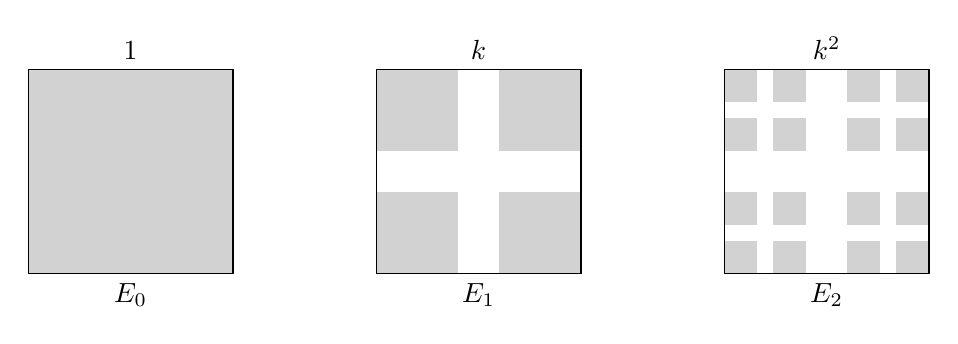
\begin{tikzpicture}[scale=2.6]
    \fill[gray!35] (0,0) rectangle (1,1);
    \draw (0,0) rectangle (1,1);
    \node[above] at (0.5,1) {$1$};
    \node[below] at (0.5,0) {$E_0$};
    \begin{scope}[xshift=1.7cm]
      \fill[gray!35] (0,0) rectangle (0.4,0.4);
      \fill[gray!35] (0.6,0) rectangle (1,0.4);
      \fill[gray!35] (0,0.6) rectangle (0.4,1);
      \fill[gray!35] (0.6,0.6) rectangle (1,1);
      \draw (0,0) grid (1,1);
      \draw (0,0) rectangle (1,1);
      \node[above] at (0.5,1) {$k$};
      \node[below] at (0.5,0) {$E_1$};
    \end{scope}
    \begin{scope}[xshift=3.4cm]
      \foreach \qx in {0,0.6} {\foreach \qy in {0,0.6} {
        \foreach \ax in {0,0.24} {\foreach \ay in {0,0.24} {
          \fill[gray!35] (\qx+\ax,\qy+\ay) rectangle ++(0.16,0.16);
        }}
      }}
      \draw (0,0) grid (1,1);
      \draw (0,0) rectangle (1,1);
      \node[above] at (0.5,1) {$k^2$};
      \node[below] at (0.5,0) {$E_2$};
    \end{scope}
  \end{tikzpicture}
  \caption{平面上一个不规则集合之构造的前几个阶段}
  \label{fig:1.2}
\end{figure}

作为替代，我们描述实直线上 Cantor 构造的一个推广.设 $s$ 是严格介于 $0$ 与 $1$ 之间的数；所构造的集合将具有维数 $s$.设 $E_0$ 表示单位区间；通过对 $E_j$ 的每个区间 $I$ 指定 $E_{j+1}\cap I$，归纳地定义集合 $E_0\supset E_1\supset E_2\cdots$，每个都是有限个闭区间之并.设 $I$ 是这样的区间，令 $m\geq 2$ 为整数，并令 $J_1,J_2,\ldots,J_m$ 为 $I$ 的等长且等距的闭子区间，其长度由
\begin{equation}\label{eq:1.23}
  |J_i|^{s}=\frac{1}{m}|I|^{s}
\end{equation}
给出，且 $J_1$ 的左端点与 $I$ 的左端点重合，$J_m$ 的右端点与 $I$ 的右端点重合.于是
\begin{equation}\label{eq:1.24}
  m|J_i|+(m-1)d=|I|\qquad(1\leq i\leq m),
\end{equation}
其中 $d$ 是相邻两个区间 $J_i$ 之间的间隔.定义 $E_{j+1}$ 使 $E_{j+1}\cap I=\bigcup_{1}^{m}J_i$.注意，$m$ 的值在 $E_j$ 的不同区间上可以不同，因此 $E_j$ 可以包含多种不同长度的区间.

集合 $E=\bigcap_{j=0}^{\infty}E_j$ 是单位区间的一个完备无处稠密子集.下述分析将出现在 Davies 即将发表的一篇文章中.

\begin{theorem}\label{thm:1.15}
若 $E$ 是如上描述的集合，则 $\mathcal{H}^s(E)=1$.
\end{theorem}

\begin{proof}
$E$ 的构造中所用的区间，即某个 $E_j$ 的分支区间，称为\newterm{net interval}{网区间}{net interval}.对 $F\subset E$，令
\begin{equation}\label{eq:1.25}
  \mu(F)=\inf\sum_{I\in\mathcal{I}}|I|^{s},
\end{equation}
其中下确界取遍 $F$ 的所有由网区间之族 $\mathcal{I}$ 构成的覆盖.则 $\mu$ 是 $E$ 的子集上的外测度（事实上还是 Borel 测度）.注意，若坚持要求 $\mathcal{I}$ 对任意 $\delta>0$ 都是 $F$ 的 $\delta$-覆盖，$\mu$ 的值并不改变，因为利用 \eqref{eq:1.23} 总可以把一个网区间 $I$ 换成若干更小的网区间而不改变 \eqref{eq:1.25} 中的和.

设 $\mathcal{I}$ 是 $E$ 的由网区间构成的覆盖.为求 $\sum_{I\in\mathcal{I}}|I|^s$ 的下界，可设族 $\mathcal{I}$ 有限（因为每个网区间相对于紧集 $E$ 是开的），还可设 $\mathcal{I}$ 中的区间两两不交（利用网的性质可去掉含于其他区间之中的那些区间）.设 $J$ 是 $\mathcal{I}$ 中最短的区间之一；设 $J$ 是某个 $E_j$ 的分支区间.则 $J\subset I$，$I$ 为 $E_{j-1}$ 中的某个区间.由于 $\mathcal{I}$ 是 $E$ 的不交覆盖，$E_j\cap I$ 的所有其他区间必都属于 $\mathcal{I}$.若把这些区间换成单个区间 $I$，则由 \eqref{eq:1.23}，$\sum|I|^s$ 的值不变.如此继续，用较大的区间替换网区间之组而不改变和的值，最终到达单个区间 $[0,1]$.于是 $\sum_{I\in\mathcal{I}}|I|^s=|[0,1]|^s=1$，特别地
\[
  \mu(E)=1.
\]
以完全相同的方式可知，若 $J$ 是任何网区间，则
\begin{equation}\label{eq:1.26}
  \mu(J\cap E)=|J|^{s}.
\end{equation}
接下来证明对任意区间 $J$ 有
\begin{equation}\label{eq:1.27}
  \mu(J\cap E)\leq|J|^{s}.
\end{equation}
必要时收缩 $J$，只需在 $J\subset[0,1]$、$J$ 的端点属于 $E$，而且（通过逼近）与含于 $J$ 中的网区间的端点重合的假设下证明.设 $I$ 是包含 $J$ 的最小网区间；设 $I$ 是某个 $E_j$ 的区间.设 $J$ 与 $E_{j+1}\cap I$ 的分支区间中的 $J_q,J_{q+1},\ldots,J_r$ 相交，其中 $1\leq q<r\leq m$.（由 $I$ 的极小性，这样的区间至少有两个.）我们断言
\begin{equation}\label{eq:1.28}
  |J_q\cap J|^{s}+|J_{q+1}|^{s}+\cdots+|J_{r-1}|^{s}+|J_r\cap J|^{s}\leq|J|^{s}.
\end{equation}
若 $J_q\cap J$ 不是整个 $J_q$，或 $J_r\cap J$ 不是整个 $J_r$，则把 $J$ 稍微放大时，\eqref{eq:1.28} 左端比右端增长得快.因此只需对 $J$ 为包含 $J_q$ 与 $J_r$ 的最小区间的情形证明 \eqref{eq:1.28}.此时 \eqref{eq:1.28} 成为
\begin{equation}\label{eq:1.29}
  k|J_i|^{s}\leq|J|^{s}=\bigl(k|J_i|+(k-1)d\bigr)^{s},
\end{equation}
其中 $k=r-q+1$.由 \eqref{eq:1.23} 与 \eqref{eq:1.24}，当 $k=m$ 时上式成立；当 $k=1$ 时显然成立且两种情形都取等号.求导两次可见 \eqref{eq:1.29} 右端作为 $k$ 的函数是凹函数\footnote{原书此处印作 ``convex function of $k$''（$k$ 的凸函数）.由于 $0<s<1$，\eqref{eq:1.29} 右端作为 $k$ 的函数实为凹函数，且论证恰好需要凹性（凹函数在区间上的最小值在端点取得），故此处按数学实际译为``凹函数''.——译者注.}，故 \eqref{eq:1.29} 对 $1\leq k\leq m$ 成立，从而 \eqref{eq:1.28} 得证.

最后，若 $J_q\cap J$ 或 $J_r\cap J$ 不是单个网区间，则可重复上述过程，把 $J_q\cap J$ 与 $J_r\cap J$ 换成更小的网区间，得到一个与 \eqref{eq:1.28} 类似但涉及 $E_{j+2}$ 而非 $E_{j+1}$ 的区间的表达式.如此继续，最终发现 $|J|^s$ 至少等于覆盖 $J\cap E$ 且含于 $J$ 内的两两不交的网区间长度之 $s$ 次幂的和.于是对任意区间 $J$，由 \eqref{eq:1.26} 即得 \eqref{eq:1.27}.

由于把 \eqref{eq:1.25} 中下确界改为取遍任意 $\delta>0$ 的 $\delta$-覆盖 $\mathcal{I}$ 时 \eqref{eq:1.25} 仍成立，故 $\mathcal{H}^s(E)\leq\mu(E)$.另一方面，由 \eqref{eq:1.27}，
\[
  \mu(E)\leq\sum\mu(J_i\cap E)\leq\sum|J_i|^{s}
\]
对 $E$ 的任何覆盖 $\{J_i\}$ 成立，故 $\mu(E)\leq\mathcal{H}^s(E)$.综上所述 $\mathcal{H}^s(E)=\mu(E)=1$.
\end{proof}

在更高维中的类似构造涉及方体或立方体的嵌套序列而非区间.同样的方法可求出 Hausdorff 维数并估计相应的 Hausdorff 测度.

\cref{thm:1.15} 的基本方法也可用于求其他相关类型集合的维数.例如，若在 $E$ 的构造中每个 $I$ 内的区间 $J_1,\ldots,J_m$ 只是``近乎相等''或``近乎等距''，该方法经调整后仍可求出 $E$ 的维数.类似地，若由 $E_j$ 得到 $E_{j+1}$ 时方程 \eqref{eq:1.23} 与 \eqref{eq:1.24} 只在``$j\to\infty$ 的极限''下成立，仍有可能求出 $E$ 的维数.

另一个求集合维数的有用技巧是把它稍加``畸变''而得到一个维数已知的集合，然后应用\cref{lem:1.8}.读者可参看\cref{thm:8.15}(a)，那里给出了示例.

\textcite{eggleston1952} 求出了由交过程形成的非常一般的集合的 Hausdorff 维数；其结果被 \textcite{peyriere1977} 推广.近来 \textcite{daviesfast1978} 描述了一种有趣而有力的方法.其他相关构造见 \textcites{randolph1941,erdos1946,ravetz1954,besicovitchtaylor1954,beardon1965,best1942,ciglervolkmann1963,wegmann1971b}，其中最后三篇是同一作者更早工作的延续.估计 Hausdorff 测度的另一种方法将在 8.3~节中描述.

\begin{exercises}
\item 证明：若 $\mu$ 是集合的 $\sigma$-域 $\mathcal{M}$ 上的测度，$E_j\in\mathcal{M}\ (1\leq j<\infty)$，则只要 $\mu\bigl(\bigcup_{1}^{\infty}E_j\bigr)<\infty$，就有
$\mu\bigl(\varlimsup_{j\to\infty}E_j\bigr)\geq\varliminf_{j\to\infty}\mu(E_j)$.
\item 设 $\nu$ 是度量空间 $(X,d)$ 上的外测度，且每个 Borel 集都 $\nu$-可测.证明 $\nu$ 是度量外测度.
\item 证明 $\mathbb{R}^n$ 上的外测度 $\mathcal{H}^s$ 平移不变，即 $\mathcal{H}^s(x+E)=\mathcal{H}^s(E)$，其中 $x+E=\{x+y:y\in E\}$.进而证明：$x+E$ 是 $\mathcal{H}^s$-可测的当且仅当 $E$ 是 $\mathcal{H}^s$-可测的.类似地，证明 $\mathcal{H}^s(cE)=c^s\mathcal{H}^s(E)$，其中 $cE=\{cy:y\in E\}$.
\item 对一般测度 $\mu$ 证明下述形式的 Vitali 覆盖定理：设 $E$ 是 $\mathbb{R}^n$ 的 $\mu$-可测子集且 $\mu(E)<\infty$.若 $\mathcal{V}$ 是 $E$ 的（由可测集构成的）Vitali 类，则存在不交集合 $U_1,U_2,\ldots\in\mathcal{V}$ 使 $\mu\bigl(E\setminus\bigcup_{i}U_i\bigr)=0$.
\item 用 Vitali 覆盖定理证明勒贝格密度定理.（对每个 $\alpha<1$ 与 $\rho>0$，考虑球类
$\mathcal{V}=\{B_r(x):x\in E,\ r\leq\rho\ \text{且}\ \mathcal{L}^n(B_r(x)\cap E)\leq\alpha\mathcal{L}^n(B_r(x))\}$.）
\item 证明直径为 $d$ 的平面凸集 $U$ 的面积至多为 $\frac{1}{4}\pi d^2$.（方法之一：取 $U$ 边界上一点为极坐标原点，使 $U$ 的面积为 $\frac{1}{2}\int r(\phi)^2\,\mathrm{d}\phi$，并注意对每个 $\phi$ 有 $r(\phi)^2+r\bigl(\phi+\frac{1}{2}\pi\bigr)^2\leq d^2$.）
\item 用勒贝格密度定理推出 \newterm{steinhaus-theorem}{Steinhaus 的结果}{Steinhaus' theorem}：若 $E$ 是测度为正的实数的勒贝格可测集，则差集 $\{y-x:x,y\in E\}$ 包含区间 $(-h,h)$.更一般地证明：若 $E$ 与 $E'$ 都是具有正勒贝格测度的可测集，则 $\{y-x:x\in E,\ y\in E'\}$ 包含一个区间.
\item 设 $\mu$ 是 $\mathbb{R}^n$ 上的 Borel 测度，$E$ 是 $\mu$-可测集且 $0<\mu(E)<\infty$.证明：(a) 若对 $x\in E$ 有 $\varlimsup_{r\to 0}r^{-s}\mu\bigl(B_r(x)\cap E\bigr)<c<\infty$，则 $\mathcal{H}^s(E)>0$；(b) 若对 $x\in E$ 有 $\varlimsup_{r\to 0}r^{-s}\mu\bigl(B_r(x)\cap E\bigr)>c>0$，则 $\mathcal{H}^s(E)<\infty$.（(a) 用 Hausdorff 测度的定义；(b) 用\cref{exe:1.4} 中形式的 Vitali 覆盖定理.）
\item 设 $E$ 是 $0$ 与 $1$ 之间其十进展开不含奇数数字的数的集合.试给出 $E$ 的 Hausdorff 维数与测度你能得到的最好上下估计.（事实上 $E$ 是一个 $s$-集，其中 $s=\log 5/\log 10$.这个例子旨在说明求 Hausdorff 测度时可能出现的一些困难，它比 Cantor 集要更棘手一些.处理此类问题的一种方法将在 8.3~节中描述.）
\end{exercises}
